% ADD/REMOVE THE 'answers' OPTION TO INCLUDE/SUPPRESS SOLUTIONS
\documentclass[11pt,addpoints,answers]{exam}
% \documentclass[11pt,addpoints,answers]{exam}

\newcommand{\hwnum}{4}
\newcommand{\duedate}{September 30}

% In order to compile this file you will need to get 'header.tex'
% and make the line below point to the appropriate file path
% Stand-in for the course-provided header.tex (EECS 376).
% It defines the macros used by hw4.tex so the file compiles on its own.
% If you have the official header.tex, just drop it in this folder instead.

\usepackage[margin=1in]{geometry}
\usepackage{amsmath,amssymb,amsthm}
\usepackage{graphicx}
\usepackage{algorithm}
\usepackage{algpseudocode}
\usepackage{enumerate}
\usepackage{xcolor}
\usepackage[colorlinks=true,linkcolor=blue,urlcolor=blue]{hyperref}

% Print "Input:" / "Output:" instead of "Require:" / "Ensure:"
\renewcommand{\algorithmicrequire}{\textbf{Input:}}
\renewcommand{\algorithmicensure}{\textbf{Output:}}

% notation macros used in the problem statements
\newcommand{\set}[1]{\left\{#1\right\}}
\newcommand{\abs}[1]{\left|#1\right|}
\newcommand{\OPT}{\mathrm{OPT}}
\newcommand{\ALG}{\mathrm{ALG}}
\newcommand{\algo}[1]{\textsc{#1}}
\newcommand{\hint}[1]{\emph{Hint:} #1}
\newcommand{\jrnote}[1]{}
\newcommand{\fxnote}[1]{}

% page headers (exam class)
\pagestyle{headandfoot}
\newcommand{\hwheader}{%
  \firstpageheader{EECS 376: Foundations of Computer Science}{}{Homework \hwnum}
  \runningheader{EECS 376: Foundations of Computer Science}{}{Homework \hwnum}
  \firstpagefooter{}{\thepage}{}
  \runningfooter{}{\thepage}{}
}
\newcommand{\hwslnheader}{%
  \firstpageheader{EECS 376: Foundations of Computer Science\\University of Michigan, Fall 2026}{}{Solutions to Homework \hwnum}
  \runningheader{EECS 376: Foundations of Computer Science\\University of Michigan, Fall 2026}{}{Solutions to Homework \hwnum}
  \firstpagefooter{}{\thepage}{}
  \runningfooter{}{\thepage}{}
}
\newcommand{\hwpreface}{%
  \noindent This homework has \numquestions{} questions, for a total of \numpoints{} points and \numbonuspoints{} extra-credit points.
  \smallskip

  \noindent Unless otherwise stated, each question requires clear, logically correct, and sufficient justification to convince the reader.
  \smallskip

  \noindent We strongly encourage you to typeset your solutions in \LaTeX.
  \smallskip

  \noindent If you collaborated with someone, you must state their name(s). You must write your own solution for all problems and may not use any other student's write-up or any AI tools.
  \bigskip
}

% solution boxes look like the posted solutions
\renewcommand{\solutiontitle}{\noindent\textbf{Solution:}\enspace}
\unframedsolutions
\pointsinrightmargin
\bracketedpoints
\marginbonuspointname{}
\bonuspointpoints{EC}{EC}

\usepackage{tikz}
\usetikzlibrary{arrows.meta,positioning}

% print "Input:"/"Output:" in pseudocode (harmless if header already does this)
\makeatletter
\@ifundefined{algorithmicrequire}{}{%
  \renewcommand{\algorithmicrequire}{\textbf{Input:}}%
  \renewcommand{\algorithmicensure}{\textbf{Output:}}}
\makeatother

\ifprintanswers
\hwslnheader   % header for solutions
\else
\hwheader   % header for homework
\fi

\begin{document}


\hwpreface

\begin{questions}

  \addtocounter{question}{-1}
  \question \textbf{Before you start; before you submit.}

      

    If applicable, state the name(s) and uniqname(s) of your collaborator(s).

    \begin{solution}
      I did not collaborate with anyone on this homework.
    \end{solution}


\question[10] \textbf{Self assessment.} \nopagebreak
  Carefully read and understand the posted solutions to the previous homework.
  Identify one part for which your own solution has the most room for improvement (e.g., has unsound reasoning, doesn’t show what was required, could be significantly clearer or better organized, etc.).
  Copy or screenshot this solution, then in a few sentences, explain what was deficient and how it could be fixed.

  (Alternatively, if you think one of your solutions is significantly \emph{better} than the posted one, copy it here and explain why you think it is better.)

  If you didn't do last week's homework, choose a problem from it that looks challenging to you, and in a few sentences, explain the key ideas behind its solution in your own words.

  \begin{solution}
    The part of HW3 with the most room for improvement is Question 2(c), the lower bound on the runtime of the recursive \algo{Count} algorithm.
    Here is what I submitted (after the pseudocode):

    \begin{quote}
      \emph{Let $T(n)$ be its running time. For $n \ge 2$, $T(n) \ge T(n-1) + T(n-2)$. This recurrence is bounded below by a constant multiple of the Fibonacci numbers, so $T(n) = \Omega(\varphi^n)$, where $\varphi = (1+\sqrt{5})/2 > 1$. The runtime is therefore exponential in $n$.}
    \end{quote}

    What was deficient: the question asked me to \emph{show} a lower bound, but I only stated one.
    The sentence ``this recurrence is bounded below by a constant multiple of the Fibonacci numbers'' is the whole argument, and I never proved it.
    Going from $T(n) \ge T(n-1)+T(n-2)$ to $T(n) = \Omega(\varphi^n)$ needs an induction (or an unrolling of the recurrence), and I skipped that step.
    So the conclusion is true, but the write-up does not justify it.

    How to fix it: the posted solution does something simpler and actually shows the work.
    Since $T$ is nondecreasing, $T(n-1) \ge T(n-2)$, so $T(n) \ge 2\,T(n-2)$.
    Unrolling this $k$ times gives $T(n) \ge 2^{k}\, T(n-2k)$, and taking $k = n/2$ gives $T(n) \ge 2^{n/2}\, T(0) = \Omega(2^{n/2})$.
    That bound is weaker than $\varphi^n$, but it is exponential in $n$, which is all the question asked for, and every step is written down.
    If I wanted to keep the $\varphi^n$ bound, I would need to prove $T(n) \ge c\,\varphi^n$ by induction using $\varphi^2 = \varphi + 1$.
  \end{solution}

\question \textbf{Fixed-color-sequence paths.} 
% \jrnote{Graph DP question from W24}
% \fxnote{In the future say the graph representation is adjacency list}
    
 
  Let $G=(V,E)$ be an undirected graph with~$n$ vertices and~$m$ edges, where $m \geq n$.
  Also, suppose that each edge is colored either black or white.
  We say that a path $P=(e_{1},\dots,e_{k})$ of edges has \emph{color sequence} $(c_{1},\dots,c_{k})$, where each $c_{i}\in\set{\text{black},\text{white}}$, if each $e_{i}$ has color $c_{i}$.
      In this problem, you will design an algorithm that, given two vertices~$s,t$ and a desired color sequence $(c_{1},\dots,c_{k})$, determines in $O(mk)$ time whether there exists a path of length $k$ from~$s$ to~$t$ with that color sequence.
  Note that paths in this problem do not need to be \emph{simple}; they can visit vertices or edges more than once.

  The graph $G=(V,E)$ is represented via \emph{adjacency lists}, i.e., for each vertex $i \in V$ there is a list of all its neighbors: vertices~$j$ such that $(i,j) \in E$.

  \begin{parts}
    \part[10]
    Derive a recurrence relation, including base case(s), for this problem.
    Briefly justify its correctness.
      
    \begin{solution}
      For $0 \le i \le k$ and a vertex $v \in V$, define
      \[
        R(i,v) = \begin{cases}
          \text{true} & \text{if there is a path of length $i$ from $s$ to $v$ with color sequence $(c_1,\dots,c_i)$,}\\
          \text{false} & \text{otherwise.}
        \end{cases}
      \]
      (A path of length $0$ is just a single vertex with no edges, and its color sequence is empty.)
      The answer to the whole problem is $R(k,t)$.

      \textbf{Base case ($i=0$).}
      The only path of length $0$ starting at $s$ is the path that stays at $s$.
      So
      \[
        R(0,v) = \begin{cases} \text{true} & \text{if } v = s,\\ \text{false} & \text{if } v \neq s. \end{cases}
      \]

      \textbf{Recursive case ($i \ge 1$).}
      \[
        R(i,v) = \bigvee_{\substack{u : (u,v) \in E \\ \text{color}(u,v) = c_i}} R(i-1,u).
      \]
      In words: $R(i,v)$ is true exactly when some neighbor $u$ of $v$, joined to $v$ by an edge of color $c_i$, has $R(i-1,u)$ true.
      (An OR over zero terms is false, so if $v$ has no incident edge of color $c_i$, then $R(i,v)$ is false.)

      \textbf{Justification.}
      I show both directions of the ``exactly when''.

      Suppose $R(i,v)$ is true, so there is a path $P = (e_1,\dots,e_i)$ from $s$ to $v$ with colors $(c_1,\dots,c_i)$.
      Its last edge $e_i = (u,v)$ has color $c_i$ for some neighbor $u$ of $v$.
      Removing $e_i$ leaves the path $(e_1,\dots,e_{i-1})$, which goes from $s$ to $u$, has length $i-1$, and has color sequence $(c_1,\dots,c_{i-1})$.
      So $R(i-1,u)$ is true, and $u$ is one of the terms in the OR.
      Hence the right-hand side is true.

      Conversely, suppose the right-hand side is true.
      Then there is a neighbor $u$ of $v$ with $\text{color}(u,v) = c_i$ and $R(i-1,u)$ true.
      Take a path of length $i-1$ from $s$ to $u$ with colors $(c_1,\dots,c_{i-1})$ and append the edge $(u,v)$.
      This gives a path of length $i$ from $s$ to $v$ with colors $(c_1,\dots,c_i)$.
      Paths do not need to be simple, so repeating a vertex or an edge is fine.
      Hence $R(i,v)$ is true.
    \end{solution}
        
    \part[6] Give pseudocode implementing an $O(km)$-time dynamic programming solution to this problem, and justify its running time.
    You do not need to give a correctness analysis since you did so for your recurrence. 
    
    \begin{solution}
      I assume each adjacency-list entry for a neighbor $u$ of $v$ also stores the color of the edge $(u,v)$, so looking up a color takes $O(1)$ time.
      (If colors are stored separately, e.g.\ in a hash table keyed by edge, the lookup is still $O(1)$.)

      \begin{algorithmic}[1]
        \Require{Adjacency lists of $G=(V,E)$ with edge colors; vertices $s,t$; colors $c_1,\dots,c_k$}
        \Ensure{true if there is a path of length $k$ from $s$ to $t$ with color sequence $(c_1,\dots,c_k)$, else false}
        \Function{ColorPath}{$G, s, t, (c_1,\dots,c_k)$}
          \State initialize a table $R[0\ldots k][V]$ of Booleans
          \For{each $v \in V$} \Comment{base case}
            \State $R[0][v] \gets \text{false}$
          \EndFor
          \State $R[0][s] \gets \text{true}$
          \For{$i = 1, \dots, k$} \Comment{fill layer $i$ from layer $i-1$}
            \For{each $v \in V$}
              \State $R[i][v] \gets \text{false}$
              \For{each neighbor $u$ in the adjacency list of $v$}
                \If{$\text{color}(u,v) = c_i$ and $R[i-1][u] = \text{true}$}
                  \State $R[i][v] \gets \text{true}$
                \EndIf
              \EndFor
            \EndFor
          \EndFor
          \State \Return $R[k][t]$
        \EndFunction
      \end{algorithmic}

      \textbf{Order of evaluation.}
      Layer $i$ of the table only uses entries from layer $i-1$, and the loop fills the layers in the order $0,1,\dots,k$.
      So every value is computed before it is needed, and the table entry $R[i][v]$ holds $R(i,v)$ from part (a).
      The answer is in $R[k][t]$.

      \textbf{Running time.}
      Filling layer $0$ takes $O(n)$ time.
      For one value of $i$, the loop over $v$ walks the entire adjacency list of every vertex.
      Each edge $(u,v)$ appears twice over all the lists (once for $u$, once for $v$), so one layer does $O(n + 2m) = O(n+m)$ work, with $O(1)$ work per list entry.
      There are $k$ layers, so the total is $O(n + k(n+m))$.
      Since $m \ge n$, this is $O(km)$.
      (The table uses $O(kn)$ space; keeping only layers $i-1$ and $i$ would reduce this to $O(n)$, since the answer only needs the last layer.)
    \end{solution}
  \end{parts}

  \question \textbf{Back to college} 
  \nopagebreak
   Michael drives down to Ann Arbor from his hometown for the start of each school year.
   Interested in minimizing his commute time, he invents a modular fuel pack for his car for the commute through various towns in Michigan.
   This fuel pack allows the vehicle to travel a certain distance before refueling.
   Each town has a service station where a fuel pack can be reloaded: the current pack is simply swapped out for a fresh full one.
   (Any remaining fuel in the removed pack will not be used by the car.)
   The goal is to visit the towns in a specified order, while minimizing the number of fuel pack reloads.

   We model this problem as follows.
   The car can travel a distance up to~$R$ on a single fuel pack.
   Starting from town 0, there are~$n$ other towns to visit in sequence.
   For $i=1, \ldots, n$, the distance from the $(i-1)$st town to the $i$th town is $d_i \leq R$.
   Given~$R$ and an array $D = [d_1, \ldots, d_n]$ as input, the goal is to find a \emph{smallest} set $S \subseteq \set{1,\ldots,n}$ of towns (specified by their indices) where refueling should occur, so that the car can reach all~$n$ towns without running out of fuel at any point.
   The car starts out with a full fuel pack, and no refueling is needed at the final town.

  \begin{parts}
    \part[7] Give a greedy algorithm (including pseuodocode) that solves this problem.
    Defer a correctness argument to the next part, but provide everything else involved in ``giving an algorithm'' here.
    
    \begin{solution}
      \textbf{Idea.}
      Starting from the current town with a full pack, drive as far as the pack allows, i.e.\ keep going while the next distance still fits in the remaining fuel.
      If the car gets to town $n$, we are done.
      Otherwise, refuel at the farthest town that was reached, and repeat from there.
      So the greedy rule is: ``always refuel as late as possible.''

      For the pseudocode I use a helper notation: for $0 \le a < b \le n$, let
      \[
        \mathrm{dist}(a,b) = d_{a+1} + d_{a+2} + \dots + d_b
      \]
      be the distance from town $a$ to town $b$.
      A set $S$ of refueling towns is \emph{valid} if every stretch between consecutive elements of $\set{0} \cup S \cup \set{n}$ has distance at most $R$.

      \begin{algorithmic}[1]
        \Require{$R > 0$ and distances $D[1\ldots n]$ with each $D[i] \le R$}
        \Ensure{A smallest valid set $S$ of refueling towns}
        \Function{GreedyRefuel}{$R, D[1\ldots n]$}
          \State $S \gets \emptyset$
          \State $i \gets 0$ \Comment{current town; the car has a full pack here}
          \While{$i < n$}
            \State $j \gets i$, $\mathit{fuel} \gets R$
            \While{$j < n$ and $\mathit{fuel} \ge D[j+1]$} \Comment{drive as far as this pack allows}
              \State $\mathit{fuel} \gets \mathit{fuel} - D[j+1]$
              \State $j \gets j+1$
            \EndWhile
            \If{$j = n$}
              \State \Return $S$ \Comment{reached the last town, no more refueling needed}
            \EndIf
            \State add $j$ to $S$ \Comment{refuel at the farthest town reached}
            \State $i \gets j$
          \EndWhile
          \State \Return $S$ \Comment{only reached when $n=0$}
        \EndFunction
      \end{algorithmic}

      \textbf{Why it always makes progress and outputs a valid set.}
      Each time the inner loop starts, $\mathit{fuel} = R \ge D[i+1]$ because every $d_i \le R$.
      So the inner loop runs at least once and $j$ ends strictly larger than $i$.
      That means $i$ strictly increases in every iteration of the outer loop, so the algorithm terminates.
      Also, by the inner loop condition, the distance from $i$ to $j$ is at most $R$, so each stretch between consecutive stops (and from the last stop to town $n$) fits in one pack.
      Hence the output is a valid set.

      \textbf{Running time.}
      The index $j$ starts at the old value of $i$ and is only ever incremented, and the next outer iteration starts $j$ from where the last one ended.
      So over the whole run, the inner loop body executes at most $n$ times in total.
      Every other operation is $O(1)$ per iteration.
      The total running time is $O(n)$.
      The extra space is $O(1)$ besides the output set.
    \end{solution}
    
    \part[10] The setup for your correctness proof is as follows.
    Let $\OPT$ be some arbitrary optimal solution.
    Let $\ALG=i_1,i_2,i_3,\dots, i_k$ be the towns chosen by your algorithm, in their greedily chosen order.
    If $\ALG = \OPT$, then $\ALG$ is optimal, as needed.
    So suppose that $\ALG \neq \OPT$, and consider the \emph{first} town $i_{\text{diff}}$ in $\ALG$ that is not in $\OPT$.
    (Such an $i_{\text{diff}}$ must exist because $\ALG$ must have at least as many towns as $\OPT$, since $\OPT$ is optimal.)
    So, $\OPT$ contains all of $i_1,i_2,i_3,\dots, i_{\text{diff}-1}$, but not $i_{\text{diff}}$.

    You will construct another optimal solution $\OPT'$ that contains all of $i_1,i_2,i_3,\ldots,i_{\text{diff}}$ by modifying $\OPT$, exchanging out some suitable town~$j$ for $i_{\text{diff}}$ instead.

    Describe which town~$j$ to exchange for $i_\text{diff}$, and prove that $\OPT'$ is an optimal solution. In particular, you should prove that $\OPT'$ is a valid solution \emph{and} an optimal solution. 
    
    \begin{solution}
      Throughout, I use $\mathrm{dist}(a,b) = d_{a+1} + \dots + d_b$ from part (a), and the following two facts.

      \begin{itemize}
        \item \textbf{Fact 1 (sub-stretches).} If $a \le a' < b' \le b$ then $\mathrm{dist}(a',b') \le \mathrm{dist}(a,b)$, because all $d_i$ are nonnegative.
        So if a stretch fits in one pack, so does any stretch inside it.
        \item \textbf{Fact 2 (what the greedy choice means).} Let $a = i_{\text{diff}-1}$, or $a = 0$ if $i_{\text{diff}} = i_1$.
        The algorithm chose $i_{\text{diff}}$ by starting at $a$ with a full pack and driving as far as possible.
        So $\mathrm{dist}(a, i_{\text{diff}}) \le R$, and since the algorithm did not stop at town $n$, we have $i_{\text{diff}} < n$ and $\mathrm{dist}(a, i_{\text{diff}}+1) > R$.
      \end{itemize}

      \textbf{Which town $j$ to exchange.}
      Let $j$ be the smallest town in $\OPT$ that is larger than $a$.
      I claim $j$ exists and $a < j < i_{\text{diff}}$.

      \emph{Existence.} $a$ is a refueling stop of $\OPT$ (or $a=0$, the start), so in $\OPT$ the car leaves $a$ with a full pack.
      If $\OPT$ had no stop in $\set{a+1,\dots,i_{\text{diff}}}$, then the car would have to drive from $a$ to some town $\ge i_{\text{diff}}+1$ (either the next stop or town $n$) on one pack.
      By Fact 1 that stretch has distance at least $\mathrm{dist}(a,i_{\text{diff}}+1) > R$, which contradicts the validity of $\OPT$.
      So $\OPT$ has a stop in $\set{a+1,\dots,i_{\text{diff}}}$, and hence $j$ exists with $a < j \le i_{\text{diff}}$.

      \emph{Strictness.} $i_{\text{diff}} \notin \OPT$ but $j \in \OPT$, so $j \ne i_{\text{diff}}$, hence $j < i_{\text{diff}}$.

      Now define
      \[
        \OPT' = (\OPT \setminus \set{j}) \cup \set{i_{\text{diff}}} .
      \]

      \textbf{$\OPT'$ contains $i_1,\dots,i_{\text{diff}}$.}
      The towns $i_1,\dots,i_{\text{diff}-1}$ are in $\OPT$ and are all $\le a < j$, so none of them is the removed town $j$.
      They stay in $\OPT'$, and $i_{\text{diff}}$ was added.

      \textbf{$\OPT'$ is valid.}
      Let $p < q$ be two consecutive elements of $\set{0} \cup \OPT' \cup \set{n}$; I show $\mathrm{dist}(p,q) \le R$.
      Note that $i_{\text{diff}} \in \OPT'$, so it is impossible that $p < i_{\text{diff}} < q$.
      That leaves two cases.

      \emph{Case $q \le i_{\text{diff}}$.}
      The town $a$ is in $\set{0}\cup\OPT'$ (it was in $\OPT$ and $a \ne j$), and $a < j < i_{\text{diff}}$, so $a < q$.
      Since $p$ is the element right before $q$, we get $p \ge a$.
      So $a \le p < q \le i_{\text{diff}}$, and by Facts 1 and 2, $\mathrm{dist}(p,q) \le \mathrm{dist}(a,i_{\text{diff}}) \le R$.

      \emph{Case $p \ge i_{\text{diff}}$.}
      Above $i_{\text{diff}}$, the sets $\OPT$ and $\OPT'$ agree, because the only changes were at $j$ and $i_{\text{diff}}$, both $\le i_{\text{diff}}$.
      \begin{itemize}
        \item If $p > i_{\text{diff}}$, then $p$ and $q$ are also consecutive in $\set{0}\cup\OPT\cup\set{n}$, so $\mathrm{dist}(p,q) \le R$ by the validity of $\OPT$.
        \item If $p = i_{\text{diff}}$, then $q$ is the smallest element of $\OPT' \cup \set{n}$ above $i_{\text{diff}}$, and since $\OPT$ and $\OPT'$ agree there, $q$ is also the smallest element of $\OPT \cup \set{n}$ above $i_{\text{diff}}$.
        Let $p'$ be the element of $\set{0}\cup\OPT$ right before $q$.
        Then $p' \ne i_{\text{diff}}$ (as $i_{\text{diff}} \notin \OPT$) and there is no element of $\OPT$ strictly between $i_{\text{diff}}$ and $q$, so $p' < i_{\text{diff}}$.
        $\OPT$ is valid, so $\mathrm{dist}(p',q) \le R$.
        Since $p' < i_{\text{diff}} < q$, Fact 1 gives $\mathrm{dist}(i_{\text{diff}},q) \le \mathrm{dist}(p',q) \le R$.
      \end{itemize}
      In all cases every stretch of $\OPT'$ has distance at most $R$, so $\OPT'$ is a valid solution.

      \textbf{$\OPT'$ is optimal.}
      We removed one town ($j \in \OPT$) and added one town ($i_{\text{diff}} \notin \OPT$), so $\abs{\OPT'} = \abs{\OPT}$.
      $\OPT'$ is valid and has the same size as an optimal solution, so $\OPT'$ is optimal.
    \end{solution}

    \part[4] Explain in your own words why the previous part (proving that $\OPT'$ is an optimal solution that contains $i_1, \ldots, i_\text{diff}$) ultimately proves that your algorithm is correct.

    \begin{solution}
      Part (b) says: if an optimal solution agrees with the greedy choices $i_1,\dots,i_{\text{diff}-1}$ but not with $i_{\text{diff}}$, we can fix it into another optimal solution that also agrees with $i_{\text{diff}}$.
      The proof only used that $\OPT$ is optimal and contains $i_1,\dots,i_{\text{diff}-1}$, so it works for any such $\OPT$ and any position $\text{diff}$.

      So we can repeat it.
      Start with any optimal solution $\OPT$.
      If it does not contain all of $i_1,\dots,i_k$, apply part (b) at the first disagreement to get an optimal solution that agrees with one more greedy town.
      Each application strictly increases the number of leading greedy towns that are contained, and there are only $k$ of them, so after at most $k$ rounds we get an optimal solution $\OPT^*$ with $\set{i_1,\dots,i_k} \subseteq \OPT^*$.
      (Formally this is an induction on $t$: for every $t \le k$ there is an optimal solution containing $i_1,\dots,i_t$.)

      Now compare sizes.
      $\ALG$ is a valid solution (shown in part (a)), so $\abs{\ALG} \ge \abs{\OPT^*}$ because $\OPT^*$ is a smallest valid solution.
      On the other hand $\ALG \subseteq \OPT^*$, so $\abs{\ALG} \le \abs{\OPT^*}$.
      Hence $\abs{\ALG} = \abs{\OPT^*}$, so $\ALG$ is optimal, i.e., the greedy algorithm always outputs a smallest valid set of refueling towns.
    \end{solution}
    
    \part[5] Now, suppose that the price of a fuel pack may differ from town to town.
    For example, a fuel pack might cost \$8 in the first town, \$3 in the second town, etc. So, the input now also includes an array $C=[c_1, \ldots, c_n]$, where~$c_i$ is the cost of refueling in the $i$th town.
    The goal now is to complete the tour while \emph{minimizing the total cost} of the fuel packs that are purchased along the way.

    Michael claims that we should use the same greedy algorithm that you proposed above to solve this problem.
    Determine whether this claim is true or not.
    \begin{itemize}
        \item If it is true, give a proof using a greedy exchange argument.
        \item Otherwise, provide a small counterexample: give a specific input, the output of your greedy algorithm on that input, and a better solution for that input; also, \emph{very briefly} explain where your proof from the previous part fails for this problem. 
    \end{itemize}
    

    \begin{solution}
      The claim is false.

      \textbf{Counterexample.}
      Take $R = 2$, $n = 3$, distances $D = [1,1,1]$, and costs $C = [1, 10, 1]$.

      \emph{Greedy output.}
      From town 0 with a full pack the car can drive $1+1 = 2 \le R$ to town 2, but not $1+1+1 = 3 > R$ to town 3.
      So the greedy algorithm refuels at town 2, then drives $1 \le R$ to town 3.
      Its output is $S = \set{2}$ with total cost $c_2 = 10$.

      \emph{Better solution.}
      $S' = \set{1}$ is valid: the stretch from 0 to 1 has distance $1 \le 2$ and the stretch from 1 to 3 has distance $1+1 = 2 \le 2$.
      Its cost is $c_1 = 1 < 10$.
      So the greedy output is not optimal.

      \textbf{Where the proof fails.}
      In part (b), $\OPT'$ was obtained from $\OPT$ by swapping $j$ for $i_{\text{diff}}$, and optimality followed from $\abs{\OPT'} = \abs{\OPT}$.
      With costs, the swap changes the objective by $c_{i_{\text{diff}}} - c_j$, which can be positive (here $c_2 - c_1 = 9$).
      So $\OPT'$ is still valid, but it can be strictly worse than $\OPT$, and the exchange step no longer produces an optimal solution.
    \end{solution}
  \end{parts}

  
  \question \textbf{Dynamic programming for dynamic shortest paths.} \nopagebreak
             
  Graphs that arise in real applications are often not fixed, but can change over time; such graphs are called ``dynamic.''
  (This is a totally different use of the word ``dynamic'' than in ``dynamic programming''.
  Computer scientists sometimes name things in confusing ways!)
  For example, roads and intersections can be added to or deleted from the road network, computers can be added to or removed from the Internet, and people can (un)follow each other on social networks.
  For many problems of interest, there are algorithms for dynamic graphs that are faster than just re-computing answers ``from scratch'' whenever the graph changes.
  In this problem you will give such algorithms for shortest-path problems.

  \vspace{1.0cm}
  
  Let $G=(V, E)$ be a weighted directed graph with $n=\abs{V}$ vertices, where the weight of each edge $(u,v)$ is denoted $w(u,v)$.
  (There can be negative-weight edges, but there is no negative-weight cycle in $G$.)
  Suppose that we have already computed the all-pairs distance table~$D$ of~$G$.
  That is, for each vertex pair $u,v \in V$, entry $D(u,v)$ stores the distance (i.e., the length of a shortest path) from~$u$ to~$v$ in $G$.

  Now, a new vertex $v_{new}$ is added to the graph, together with its incident edges.
  Let $G_{new} = (V \cup \set{v_{new}}, E \cup E_{new})$ denote the updated graph, where $E_{new}$ consists of all the incoming and outgoing edges for $v_{new}$.
  (There is no negative-weight cycle in $G_{new}$.)
  We aim to compute the updated distance table $D_{new}$ of~$G_{new}$.

  A straightforward approach is to compute $D_{new}$ from scratch using the Floyd-Warshall algorithm, in $\Theta(n^3)$ time.
  But we want to do better by exploiting the fact that we already have~$D$.
  In this problem, you will obtain a faster $O(n^2)$-time algorithm.

  \begin{parts}
    
    \part[10] Write expressions for $D_{new}(v_{new},u)$ and $D_{new}(u,v_{new})$ that hold for all $u\in V$, where the expressions are in terms of the already-known quantities $D(y,z)$ for $y,z\in V$, and $w(y,z)$ for $(y,z) \in E \cup E_{new}$. 
    Evaluating your expressions should take $O(n)$ time for each vertex~$u$, for a total of $O(n^2)$ time.
    Justify the correctness of your expressions and the evaluation time.
    
    \hint{Consider why the Bellman-Ford algorithm is correct.}
    
    \begin{solution}
      Conventions: $D(y,z) = \infty$ if there is no path from $y$ to $z$, $D(y,y) = 0$, and the minimum over an empty set is $\infty$.
      I also use the standard fact that in a graph with no negative-weight cycle, for every $u,v$ with a path from $u$ to $v$ there is a shortest path that is \emph{simple}: given any walk from $u$ to $v$, repeatedly cut out a cycle; this never increases the length because every cycle has weight $\ge 0$.

      \textbf{Expressions.}
      For every $u \in V$,
      \begin{align*}
        D_{new}(v_{new},u) &= \min_{x : (v_{new},x) \in E_{new}} \bigl( w(v_{new},x) + D(x,u) \bigr), \\
        D_{new}(u,v_{new}) &= \min_{y : (y,v_{new}) \in E_{new}} \bigl( D(u,y) + w(y,v_{new}) \bigr).
      \end{align*}
      (Also $D_{new}(v_{new},v_{new}) = 0$.)

      \textbf{Correctness of the first expression.}
      Fix $u \in V$ and let $M$ be the right-hand side.

      \emph{$D_{new}(v_{new},u) \le M$.}
      If $M = \infty$ there is nothing to show.
      Otherwise take an out-edge $(v_{new},x)$ attaining the minimum, so $D(x,u) < \infty$.
      Take a shortest path from $x$ to $u$ in $G$ (length $D(x,u)$) and put the edge $(v_{new},x)$ in front of it.
      This is a walk from $v_{new}$ to $u$ in $G_{new}$ of length $w(v_{new},x) + D(x,u) = M$.
      By the fact above, there is a path of length at most $M$, so $D_{new}(v_{new},u) \le M$.

      \emph{$D_{new}(v_{new},u) \ge M$.}
      If $D_{new}(v_{new},u) = \infty$ there is nothing to show.
      Otherwise take a simple shortest path $P$ from $v_{new}$ to $u$ in $G_{new}$.
      Since $u \ne v_{new}$, $P$ has at least one edge, and its first edge is some $(v_{new},x) \in E_{new}$.
      Since $P$ is simple, $v_{new}$ does not appear again, so the rest of $P$ is a path from $x$ to $u$ that uses only vertices of $V$ and edges of $E$.
      Its length is at least $D(x,u)$.
      Hence
      \[
        D_{new}(v_{new},u) = \text{len}(P) \ge w(v_{new},x) + D(x,u) \ge M.
      \]
      This is the same idea as the Bellman-Ford relaxation step: a shortest path to $u$ is an edge out of the source followed by a shortest path from the other endpoint.

      \textbf{Correctness of the second expression.}
      This is symmetric.
      A simple shortest path from $u$ to $v_{new}$ in $G_{new}$ has $v_{new}$ only as its last vertex, so its last edge is some $(y,v_{new}) \in E_{new}$ and the part before it is a path from $u$ to $y$ inside $G$, of length at least $D(u,y)$.
      That gives $D_{new}(u,v_{new}) \ge \min_y (D(u,y) + w(y,v_{new}))$.
      Conversely, a shortest $u$-to-$y$ path in $G$ followed by the edge $(y,v_{new})$ is a walk of length $D(u,y) + w(y,v_{new})$, and it can be shortened to a path, so $D_{new}(u,v_{new}) \le \min_y(D(u,y)+w(y,v_{new}))$.

      \textbf{Evaluation time.}
      $v_{new}$ has at most $n$ out-edges and at most $n$ in-edges, so each minimum ranges over at most $n$ terms.
      Each term is a table lookup plus an addition, which is $O(1)$.
      So each of the two values takes $O(n)$ time for a fixed $u$, and computing them for all $n$ vertices $u$ takes $O(n^2)$ time in total.
    \end{solution}

    \part[8] Write an expression for $D_{new}(u,v)$ that holds for all $u,v \in V$, where the expression is in terms of the already-known quantities listed in the previous part, as well as the quantities you computed in the previous part.
    Evaluating your expression for all $u,v \in V$ should take a total of $O(n^2)$ time.
    Justify the correctness of your expression and the evaluation time.

    Observe that by combining the two parts, we have computed the entire new distance table $D_{new}$ of $G_{new}$ in $O(n^2)$ time!
    
    \hint{Consider why the Floyd-Warshall algorithm is correct.}

    \begin{solution}
      \textbf{Expression.}
      For all $u,v \in V$,
      \[
        D_{new}(u,v) = \min\set{\, D(u,v),\ \ D_{new}(u,v_{new}) + D_{new}(v_{new},v) \,},
      \]
      where the two $D_{new}$ terms on the right are the values computed in part (a).

      This is exactly one round of Floyd-Warshall with $v_{new}$ as the last ``intermediate'' vertex: a shortest path either does not go through $v_{new}$, or it does, and then it splits into a shortest path to $v_{new}$ and a shortest path from $v_{new}$.

      \textbf{Correctness.}
      Fix $u,v \in V$ and let $M$ be the right-hand side.

      \emph{$D_{new}(u,v) \le M$.}
      First, every path in $G$ is also a path in $G_{new}$, so $D_{new}(u,v) \le D(u,v)$.
      Second, if both $D_{new}(u,v_{new})$ and $D_{new}(v_{new},v)$ are finite, then a shortest path from $u$ to $v_{new}$ followed by a shortest path from $v_{new}$ to $v$ is a walk from $u$ to $v$ in $G_{new}$ of length $D_{new}(u,v_{new}) + D_{new}(v_{new},v)$.
      Since $G_{new}$ has no negative cycle, this walk can be shortened to a path with no larger length, so $D_{new}(u,v) \le D_{new}(u,v_{new}) + D_{new}(v_{new},v)$.
      Together, $D_{new}(u,v) \le M$.

      \emph{$D_{new}(u,v) \ge M$.}
      If $D_{new}(u,v) = \infty$ we are done.
      Otherwise take a simple shortest path $P$ from $u$ to $v$ in $G_{new}$.
      \begin{itemize}
        \item If $P$ does not visit $v_{new}$, then $P$ only uses vertices of $V$ and edges of $E$, so it is a path in $G$ and $\text{len}(P) \ge D(u,v) \ge M$.
        \item If $P$ visits $v_{new}$, it does so exactly once because $P$ is simple.
        Split $P$ at $v_{new}$ into $P_1$ (from $u$ to $v_{new}$) and $P_2$ (from $v_{new}$ to $v$).
        Both are paths in $G_{new}$, so $\text{len}(P_1) \ge D_{new}(u,v_{new})$ and $\text{len}(P_2) \ge D_{new}(v_{new},v)$.
        Hence $\text{len}(P) = \text{len}(P_1) + \text{len}(P_2) \ge D_{new}(u,v_{new}) + D_{new}(v_{new},v) \ge M$.
      \end{itemize}
      In both cases $D_{new}(u,v) = \text{len}(P) \ge M$.

      \textbf{Evaluation time.}
      After part (a), the values $D_{new}(u,v_{new})$ and $D_{new}(v_{new},v)$ are stored for every $u$ and $v$.
      So for each pair $(u,v)$ the expression is three table lookups, one addition and one minimum, i.e.\ $O(1)$ time.
      There are $n^2$ pairs, so the total is $O(n^2)$.
      Together with the $O(n^2)$ time of part (a), the whole table $D_{new}$ (including the row and column of $v_{new}$) is computed in $O(n^2)$ time.
    \end{solution}
  \end{parts}  



  \question \textbf{MST mashup.} \nopagebreak 
  
  \begin{parts}
    
    \part[5] Consider the following claim: a minimum spanning tree in a graph is \emph{unique} if the edge weights are \emph{distinct} (all different).

    Professor $\Upsilon$ presents you with the following bogus ``proof'' of this claim: \emph{because edge weights are distinct, all choices in Kruskal's algorithm are completely determined---there are no ``ties'' between edge weights that the algorithm can choose how to break.
      So, the algorithm has only one possible output.
      Because Kruskal's algorithm is correct for the MST problem, its unique output must be the only minimum spanning tree in the graph.}
      
    Briefly explain what is wrong with this ``proof.''
    In particular, indicate which sentence in the ``proof'' does not follow from the previous one, and provide a reason for it.

    \begin{solution}
      The first two sentences are fine: with distinct weights, Kruskal's algorithm is deterministic and has a single possible output.

      The third sentence does not follow from the second.
      ``Kruskal's algorithm is correct'' means that its output is \emph{some} minimum spanning tree.
      It does not say that \emph{every} minimum spanning tree is an output of Kruskal's algorithm.
      So ``the algorithm has one output'' plus ``that output is an MST'' does not rule out other MSTs that the algorithm simply never produces.

      Here is why this kind of reasoning is invalid in general.
      Take a triangle whose three edges all have weight 1, and run Kruskal's algorithm with a fixed tie-breaking rule (say, by edge index).
      Then the algorithm is deterministic and has exactly one output, and it is correct, so its output is an MST.
      But the triangle has three different MSTs (drop any one edge).
      So ``deterministic and correct'' by itself never implies uniqueness of the optimum.
      The claim happens to be true for distinct weights, but it needs a real argument about the weights, which is part (b).
    \end{solution}

    \part[8]
    Give a correct proof for the claim in the previous part.
    
    \hint{Consider two distinct spanning trees $T_1, T_2$ and prove via an exchange argument that one of them does not have minimum weight.}

    \begin{solution}
      Let $G$ be a connected graph with distinct edge weights, and suppose for contradiction that $T_1 \ne T_2$ are both minimum spanning trees of $G$.

      \textbf{Choosing the edge to exchange.}
      Since $T_1 \ne T_2$ and both are sets of edges, the symmetric difference $T_1 \triangle T_2 = (T_1 \setminus T_2) \cup (T_2 \setminus T_1)$ is nonempty.
      Let $e$ be the edge of minimum weight in $T_1 \triangle T_2$; it is unique since weights are distinct.
      By symmetry (swap the names of $T_1$ and $T_2$ if needed), assume $e \in T_1 \setminus T_2$.

      \textbf{Finding a heavier edge $f$ in $T_2$.}
      $T_2$ is a spanning tree, so its two endpoints of $e$ are connected by a path in $T_2$.
      Adding $e$ to $T_2$ therefore creates a cycle $C$ in $T_2 \cup \set{e}$, and $e \in C$.
      Not every edge of $C$ can be in $T_1$: otherwise $C$ would be a cycle inside the tree $T_1$, which is impossible.
      So $C$ has some edge $f \notin T_1$.
      Since $f \ne e$ (as $e \in T_1$) and every edge of $C$ other than $e$ lies in $T_2$, we get $f \in T_2 \setminus T_1 \subseteq T_1 \triangle T_2$.
      By the choice of $e$ as the unique lightest edge of $T_1 \triangle T_2$, and since $f \ne e$,
      \[
        w(f) > w(e).
      \]

      \textbf{The exchange.}
      Let $T_2' = (T_2 \setminus \set{f}) \cup \set{e}$.
      I claim $T_2'$ is a spanning tree.
      Removing $f$ from the cycle $C$ in $T_2 \cup \set{e}$ keeps the graph connected: any path that used $f$ can go around the rest of $C$ instead.
      So $T_2'$ is connected, spans all $n$ vertices, and has $(n-1) - 1 + 1 = n-1$ edges.
      A connected graph on $n$ vertices with $n-1$ edges is a tree, so $T_2'$ is a spanning tree.

      Its weight is
      \[
        w(T_2') = w(T_2) - w(f) + w(e) < w(T_2),
      \]
      which contradicts the assumption that $T_2$ is a minimum spanning tree.

      So two distinct minimum spanning trees cannot exist, i.e., the MST is unique when the edge weights are distinct.
    \end{solution}

  \end{parts}


  \question \textbf{Greedy knapsack filling.} \nopagebreak
    
  Recall the knapsack problem (sometimes called the ``0-1'' knapsack problem): you are given~$n$ items, where the $i$th item has weight~$w_{i}$ and value~$v_{i}$ (both positive integers), and a non-negative weight capacity~$C$ of the knapsack.
  An optimal solution is a subset $S\subseteq \set{1, 2, \ldots, n}$ of the items having maximum total value \[ \sum_{i\in S} v_i \; \text, \] under the constraint that the total weight is at most the knapsack capacity, i.e., \[ \sum_{i\in S} w_i \leq C \; \text. 
  \]

  In this problem, we introduce the \emph{fractional} variant of the knapsack problem, where one may take any fraction $p_i \in [0,1]$ of any item~$i$.
  Naturally, a $p_i$-fraction of item~$i$ weighs $p_i \cdot w_i$, and has value $p_i \cdot v_i$.
  The goal is to maximize the total value of the selected fractional items.

  \begin{parts}

    \part[2] 
    Briefly explain why the optimal value for the fractional knapsack problem is \emph{at least as large} as that of the original 0-1 knapsack problem (for the same weights, values, and knapsack capacity).

    \begin{solution}
      Every feasible solution of the 0-1 problem is also a feasible solution of the fractional problem with the same value.
      Given a subset $S$ with $\sum_{i \in S} w_i \le C$, set $p_i = 1$ for $i \in S$ and $p_i = 0$ otherwise.
      Then every $p_i \in [0,1]$, the total weight $\sum_i p_i w_i = \sum_{i\in S} w_i \le C$ is feasible, and the total value $\sum_i p_i v_i = \sum_{i \in S} v_i$ is the same.
      In particular, an optimal 0-1 solution gives a feasible fractional solution of the same value.
      The fractional optimum is the maximum over a set of solutions that contains this one, so it is at least the 0-1 optimum.
    \end{solution}
    
    \part[5] Consider the following two greedy algorithms for the fractional knapsack problem:
    \begin{itemize}
    \item \algo{ValueGreedy}: While there is still some unused knapsack capacity and at least one unconsidered item, choose an item having the \emph{largest value} (among those not considered yet), and add the largest possible fraction of that item (up to the entire item) that will fit within the remaining knapsack capacity.
        
    \item \algo{WeightGreedy}: While there is still some unused knapsack capacity and at least one unconsidered item, choose an item having the \emph{smallest weight} (among those not considered yet), and add the largest possible fraction of that item (up to the entire item) that will fit within the remaining knapsack capacity.
    \end{itemize}

    Suppose we run \emph{both} algorithms \algo{ValueGreedy} and \algo{WeightGreedy}, and output a best one of their two outputs.
    Is this a correct algorithm for the fractional knapsack problem?
    If so, prove it.
    Otherwise, give an input for which this algorithm's output is not optimal, and show why it is not.

    \begin{solution}
      No, it is not correct.
      Here is an input with capacity $C = 3$ and three items:
      \[
        \begin{array}{c|ccc}
          \text{item} & 1 & 2 & 3 \\ \hline
          w_i & 1 & 2 & 3 \\
          v_i & 1 & 4 & 5
        \end{array}
      \]
      (There are no ties in value or weight, so both algorithms are fully determined.)

      \textbf{\algo{ValueGreedy}.}
      The largest value is $v_3 = 5$.
      Item 3 has weight $3 \le C$, so the whole item fits and the capacity drops to $0$.
      The algorithm stops with total value $5$.

      \textbf{\algo{WeightGreedy}.}
      The smallest weight is $w_1 = 1$; take all of item 1 (value 1, capacity left $2$).
      Next smallest is $w_2 = 2$; take all of item 2 (value 4, capacity left $0$).
      The algorithm stops with total value $1 + 4 = 5$.

      So the best of the two outputs has value $5$.

      \textbf{A better solution.}
      Take all of item 2 and one third of item 3: $p = (0, 1, \tfrac13)$.
      The weight is $2 + \tfrac13 \cdot 3 = 3 \le C$, so it is feasible, and the value is $4 + \tfrac13 \cdot 5 = \tfrac{17}{3} > 5$.
      Hence the combined algorithm's output is not optimal.

      (Intuitively, item 2 has the best value per unit weight, $v_2/w_2 = 2$, but it is neither the most valuable nor the lightest item, so neither greedy rule looks at it first.)
    \end{solution}

    \part[10] Consider the following greedy algorithm for the fractional knapsack problem: 
    \begin{itemize}
    \item \algo{RelativelyGreedy}: While there is still some unused knapsack capacity, choose an item having the largest \emph{relative value} $v_i/w_i$ (among those not considered yet), and add the largest possible fraction of that item (up to the full item) that will fit within the remaining knapsack capacity.
    \end{itemize}

    In this part, you will prove that the \algo{RelativelyGreedy} algorithm is a correct algorithm for the fractional knapsack problem.
    This is notable because we used a more complicated dynamic programming algorithm to solve 0-1 Knapsack, but the fractional variant admits a much simpler greedy algorithm!

    The setup for your correctness proof is as follows.
    Without loss of generality, suppose that the items are in sorted order by relative value $r_{i}=v_{i}/w_{i}$, from largest to smallest (the algorithm considers them in this order).
    Let $\ALG=p_1,p_2,\dots,p_n$ be the fractions of items $1,2,\dots, n$ chosen by the algorithm, respectively.
    (So, $p_i=1$ if the algorithm chooses all of item~$i$, and $p_i=0$ if it doesn't choose any of item~$i$.)

    Let $\OPT$ be an arbitrary optimal solution.
    If $\ALG = \OPT$, then $\ALG$ is optimal, as needed.
    So suppose that $\ALG \neq \OPT$, and consider the smallest index $j$ such that $\OPT$ does not have \emph{exactly} a $p_j$-fraction of item $j$.

    You will construct another solution $\OPT'$ whose fractions of the first~$j$ items are exactly $p_1,p_2,\ldots,p_j$ by modifying $\OPT$, using an exchange argument.

    Describe which fraction(s) of item(s) to exchange, and prove that $\OPT'$ is an optimal solution; this should include a proof that $\OPT'$ is a \emph{valid} solution.

    \begin{solution}
      Write $\OPT = q_1,\dots,q_n$ for the fractions in $\OPT$.
      By the choice of $j$, $q_i = p_i$ for all $i < j$ and $q_j \ne p_j$.
      Let
      \[
        W = \sum_{i<j} p_i w_i = \sum_{i<j} q_i w_i
      \]
      be the weight both solutions put on the first $j-1$ items.

      \textbf{Step 1: $q_j < p_j$.}
      When the algorithm reached item $j$, its remaining capacity was $C - W$ (if this was $0$ the algorithm had already stopped, and then $p_j = 0$).
      It took the largest fraction that fits, so
      \[
        p_j = \min\set{1,\ \tfrac{C-W}{w_j}}.
      \]
      $\OPT$ is feasible, so $W + q_j w_j \le C$, i.e.\ $q_j \le \frac{C-W}{w_j}$; also $q_j \le 1$.
      So $q_j \le \min\set{1, \frac{C-W}{w_j}} = p_j$.
      Since $q_j \ne p_j$, we get $q_j < p_j$.

      \textbf{Step 2: which fractions to exchange.}
      Let $\delta = p_j - q_j > 0$, and let $\Delta = \delta w_j$ be the extra weight of item $j$ we want to add.
      Let $L = \sum_{i > j} q_i w_i$ be the weight $\OPT$ puts on items after $j$, and let $F = C - W - q_j w_j - L \ge 0$ be the unused capacity of $\OPT$.
      Since $p_j w_j \le C - W$ (from Step 1),
      \[
        \Delta = p_j w_j - q_j w_j \le C - W - q_j w_j = L + F .
      \]
      So there is enough room to add $\Delta$ if we use the free capacity first and then remove weight from later items.
      Concretely, let $\Delta' = \max\set{0, \Delta - F}$ be the weight that must be removed from items $j+1,\dots,n$; note $0 \le \Delta' \le L$.
      Go through $i = j+1, j+2, \dots, n$ and remove from item $i$ a weight $x_i$ with $0 \le x_i \le q_i w_i$, taking as much as possible from each item until the removed weights add up to exactly $\Delta'$.
      This is possible because $\Delta' \le L = \sum_{i>j} q_i w_i$.
      Define $\OPT' = q'_1,\dots,q'_n$ by
      \[
        q'_i = q_i \ (i<j), \qquad q'_j = p_j, \qquad q'_i = q_i - \frac{x_i}{w_i} \ (i>j).
      \]
      In words: add a $\delta$-fraction of item $j$, and pay for it with unused capacity and with fractions of lower-density items.

      \textbf{Step 3: $\OPT'$ is valid.}
      Every fraction is in $[0,1]$: for $i<j$ nothing changed; $q'_j = p_j \in [0,1]$; and for $i > j$, $0 \le x_i \le q_i w_i$ gives $0 \le q'_i \le q_i \le 1$.
      The total weight is
      \[
        \sum_i q'_i w_i
        = W + (q_j + \delta) w_j + (L - \Delta')
        = \underbrace{(W + q_j w_j + L)}_{=\,C - F} + \Delta - \Delta'
        = C - F + \min\set{\Delta, F} \le C .
      \]
      So $\OPT'$ is a valid solution.

      \textbf{Step 4: $\OPT'$ is optimal.}
      The change in value is
      \[
        \text{val}(\OPT') - \text{val}(\OPT) = \delta v_j - \sum_{i>j} \frac{x_i}{w_i} v_i = \Delta\, r_j - \sum_{i>j} x_i\, r_i .
      \]
      The items are sorted by relative value, so $r_i \le r_j$ for every $i > j$, and every $x_i \ge 0$.
      Therefore
      \[
        \sum_{i>j} x_i r_i \le r_j \sum_{i>j} x_i = r_j \Delta' \le r_j \Delta,
      \]
      so $\text{val}(\OPT') - \text{val}(\OPT) \ge 0$.
      Thus $\OPT'$ is a valid solution with value at least that of $\OPT$.
      Since $\OPT$ is optimal, $\OPT'$ cannot have larger value, so $\text{val}(\OPT') = \text{val}(\OPT)$ and $\OPT'$ is optimal.

      Finally, $\OPT'$ has fractions $p_1,\dots,p_{j-1}$ on the first $j-1$ items (unchanged from $\OPT$) and $p_j$ on item $j$, as required.
      Repeating this exchange at each disagreement (as in Question 3(c)) gives an optimal solution equal to $\ALG$, so \algo{RelativelyGreedy} is correct.
    \end{solution}

  \end{parts}
  

  \bonusquestion \textbf{Optional extra credit: Greedily independent.} 

  
  \nopagebreak

  An \emph{independent set} of an undirected graph $G=(V,E)$ is a subset of vertices $S \subseteq V$ such that no two vertices in $S$ are adjacent, i.e., $(u,v) \notin E$ for every distinct $u,v \in S$.
  We are interested in a \emph{maximum} independent set, i.e., the independent set with the \emph{largest} number of vertices.
  (There may be more than one maximum independent set.)
    
  Consider the following greedy algorithm for finding an independent set in a graph.

  \begin{minipage}{\linewidth}
    \begin{algorithm}[H]
      \begin{algorithmic}[1]
        \Function{GreedyIS}{$G=(V,E)$}
        \State{$S \gets \emptyset$}
        \While{$G$ has at least one vertex}
            \State{Select any vertex~$v$ in $G$ that has \emph{smallest} degree (i.e., the fewest neighbors)}
            \State{Add $v$ to $S$}
            \State{Remove $v$ and all its neighbors, including all their incident edges, from $G$}
        \EndWhile
        \State{\Return{$S$}}
        \EndFunction
      \end{algorithmic}
    \end{algorithm}
  \end{minipage}

  \begin{parts}

    \bonuspart[1]
    
    Give an example of a graph for which the algorithm \algo{GreedyIS} \textbf{does not} return the maximum independent set.
    You can assign numbers to the vertices of your graph, and assume that in the case where there are multiple vertices with the smallest degree, \algo{GreedyIS} will choose the vertex having the smallest number. 
    \begin{solution}
      Take the graph with vertices $1,\dots,6$ and edges
      \[
        (1,2),\ (1,3),\ (2,4),\ (3,4),\ (4,5),\ (4,6),\ (5,6).
      \]
      It is a 4-cycle $1\!-\!2\!-\!4\!-\!3\!-\!1$ glued to a triangle $4\!-\!5\!-\!6$ at vertex $4$.

      \begin{center}
        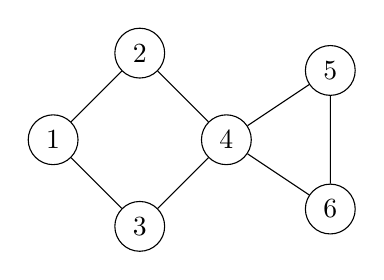
\begin{tikzpicture}[every node/.style={circle,draw,inner sep=2pt,minimum size=18pt},scale=1.1]
          \node (1) at (0,0) {1};
          \node (2) at (1,1) {2};
          \node (3) at (1,-1) {3};
          \node (4) at (2,0) {4};
          \node (5) at (3.2,0.8) {5};
          \node (6) at (3.2,-0.8) {6};
          \draw (1)--(2) (1)--(3) (2)--(4) (3)--(4) (4)--(5) (4)--(6) (5)--(6);
        \end{tikzpicture}
      \end{center}

      \textbf{Run of \algo{GreedyIS}.}
      The degrees are $\deg(1)=\deg(2)=\deg(3)=\deg(5)=\deg(6)=2$ and $\deg(4)=4$.
      The smallest degree is $2$, and the smallest-numbered vertex with that degree is $1$.
      So the algorithm adds $1$ to $S$ and removes $1$ and its neighbors $2,3$.
      The remaining graph is the triangle on $4,5,6$, where every vertex has degree $2$, so the algorithm picks $4$ and removes $4,5,6$.
      Nothing is left, and it returns $S = \set{1,4}$, of size $2$.

      \textbf{A larger independent set.}
      $\set{2,3,5}$ is independent: none of $(2,3)$, $(2,5)$, $(3,5)$ is an edge.
      It has size $3 > 2$, so the output of \algo{GreedyIS} is not a maximum independent set.
    \end{solution}

    
    \bonuspart[2] In this part, you will prove that \algo{GreedyIS} returns a maximum independent set when the input graph is a \emph{tree}.

    The setup for the proof is as follows.
    Let $\ALG=v_1,v_2,v_3,\dots,v_k$ be the vertices chosen by your algorithm, in their greedily chosen order, and let $\OPT$ be some arbitrary optimal solution.
    If $\ALG = \OPT$, then $\ALG$ is optimal, as needed.
    So suppose that $\ALG \neq \OPT$, and consider the \emph{first} vertex $v_{\text{diff}}$ in $\ALG$ that is not in $\OPT$.
    (Such a $v_{\text{diff}}$ must exist because $\ALG$ cannot be a proper subset of $\OPT$; do you see why?)
    So, $\OPT$ contains all of $v_1,v_2,v_3,\dots,v_{\text{diff}-1}$, but not $v_{\text{diff}}$.
    
    You will construct another optimal solution (a maximum independent set) $\OPT'$ that has all of $v_1,v_2,v_3,\ldots,v_{\text{diff}}$ by modifying $\OPT$, exchanging out some suitable vertex~$u$ for $v_{\text{diff}}$ instead.

    Describe which vertex~$u$ to exchange for $v_\text{diff}$, and prove that $\OPT'$ is both valid \textit{and} optimal.

    \begin{solution}
      (Why $v_{\text{diff}}$ exists: $\ALG$ is a \emph{maximal} independent set, since every vertex not in $\ALG$ was removed as a neighbor of some chosen vertex.
      So no independent set strictly contains $\ALG$, and in particular $\ALG$ is not a proper subset of $\OPT$.)

      Let $d = \text{diff}$, and let $G_d$ be the graph that remains right before the algorithm picks $v_d$.
      Two observations about $G_d$:

      \begin{itemize}
        \item \textbf{(O1) $G_d$ is a forest.} It is obtained from the tree $G$ by deleting vertices, and any subgraph of a tree has no cycles.
        \item \textbf{(O2) The vertices deleted before step $d$ are exactly $v_1,\dots,v_{d-1}$ and their neighbors in $G$, and none of these neighbors is in $\OPT$.}
        The first claim is just what the algorithm does.
        For the second: $\OPT$ contains $v_1,\dots,v_{d-1}$ and is independent, so it contains no neighbor of any $v_i$ with $i<d$.
      \end{itemize}
      A consequence of (O2): $v_d$ is in $G_d$, so it is not adjacent (in $G$) to any of $v_1,\dots,v_{d-1}$; otherwise it would have been deleted earlier.
      So every neighbor of $v_d$ in $G$ that is \emph{not} in $G_d$ is a neighbor of some $v_i$ ($i<d$), and hence is not in $\OPT$.

      \textbf{Which vertex $u$ to exchange.}
      By (O1), $G_d$ is a forest, so it has a vertex of degree $0$ or $1$ (every tree with at least two vertices has a leaf).
      The algorithm picks a vertex of smallest degree, so $v_d$ has degree $0$ or $1$ in $G_d$.

      \emph{Degree $0$ cannot happen.}
      If $v_d$ had no neighbors in $G_d$, then by the consequence of (O2) all its neighbors in $G$ lie outside $\OPT$.
      Then $\OPT \cup \set{v_d}$ would be an independent set larger than $\OPT$ (recall $v_d \notin \OPT$), contradicting that $\OPT$ is maximum.

      So $v_d$ has exactly one neighbor in $G_d$; call it $u$.
      Define
      \[
        \OPT' = (\OPT \setminus \set{u}) \cup \set{v_d}.
      \]

      \textbf{$u$ is in $\OPT$.}
      Suppose not.
      The neighbors of $v_d$ in $G$ are $u$ and vertices outside $G_d$; the latter are not in $\OPT$ by the consequence of (O2), and $u \notin \OPT$ by assumption.
      So $v_d$ has no neighbor in $\OPT$, and $\OPT \cup \set{v_d}$ is an independent set of size $\abs{\OPT}+1$, a contradiction.
      Hence $u \in \OPT$.

      \textbf{$\OPT'$ is valid (independent).}
      Take two distinct vertices $x,y \in \OPT'$.
      If neither is $v_d$, then both are in $\OPT$, so they are not adjacent.
      If $x = v_d$, then $y \in \OPT \setminus \set{u}$.
      The only neighbors of $v_d$ are $u$ (removed) and vertices outside $\OPT$, so $y$ is not adjacent to $v_d$.
      So $\OPT'$ is an independent set.

      \textbf{$\OPT'$ is optimal.}
      We removed $u \in \OPT$ and added $v_d \notin \OPT$, so $\abs{\OPT'} = \abs{\OPT}$.
      An independent set of the same size as a maximum independent set is itself maximum.

      \textbf{$\OPT'$ contains $v_1,\dots,v_d$.}
      The vertex $u$ lies in $G_d$, while $v_1,\dots,v_{d-1}$ were deleted before step $d$, so $u \ne v_i$ for all $i<d$.
      Hence $v_1,\dots,v_{d-1}$ stay in $\OPT'$, and $v_d$ was added.

      Repeating this exchange at each disagreement (exactly as in Question 3(c)) yields a maximum independent set that contains all of $v_1,\dots,v_k$.
      Since $\ALG$ is a maximal independent set, that set must equal $\ALG$, so \algo{GreedyIS} returns a maximum independent set on every tree.
    \end{solution}

  \end{parts}




\end{questions}
\end{document}
